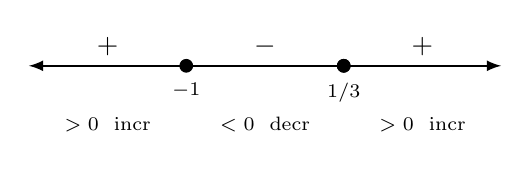
\begin{tikzpicture}[>=latex]

\draw [<->, thick] (-3,0) -- (3,0);
\foreach \x / \y  in %
					{%
					-1/{$-1$},%
					1/{$1/3$},%
					}
		{\draw [fill] (\x,0) circle [radius=0.08];
		 \draw (\x,-0.1) node[below] {\scriptsize \parbox{40pt}{\centering \y}};}
		
\draw (-2,-.75) node {\scriptsize \parbox{50pt}{\centering $\fp>0$ \ incr }};
\draw (0,-.75) node {\scriptsize \parbox{50pt}{\centering $\fp<0$ \ decr }};
\draw (2,-.75) node {\scriptsize \parbox{50pt}{\centering $\fp>0$ \ incr }};
\draw (-2,.25) node {$+$};
\draw (0,.25) node {$-$};
\draw (2,.25) node {$+$};
%\draw (3.75,.5) node {\scriptsize \parbox{50pt}{\centering $\fp>0$ \ incr \vskip 3pt $\fpp<0$ \ c. up}};


\end{tikzpicture}